%!TEX root = ../Thesis.tex
\section{Step 1}
The system given has the cars driving around the circuit in their specific routes. The cars does not stop, when they bump into each other, instead a red square is shown for each collision.
\\

Step one's requirements are to
\begin{itemize}
\item make sure the cars do not collide
\item cause deadlocks in the traffic
\item have cars drive through the alley
\end{itemize}

\subsection{Avoid collision}
Overall the challenges is to stop the cars' collisions and have semaphores handle the alley. The deadlocks is a part in both the collision and the alley in a way.

\begin{figure}[H]
\centering
\caption{The cars driving around the parking lot}
\begin{subfigure}[b]{0.4\textwidth}
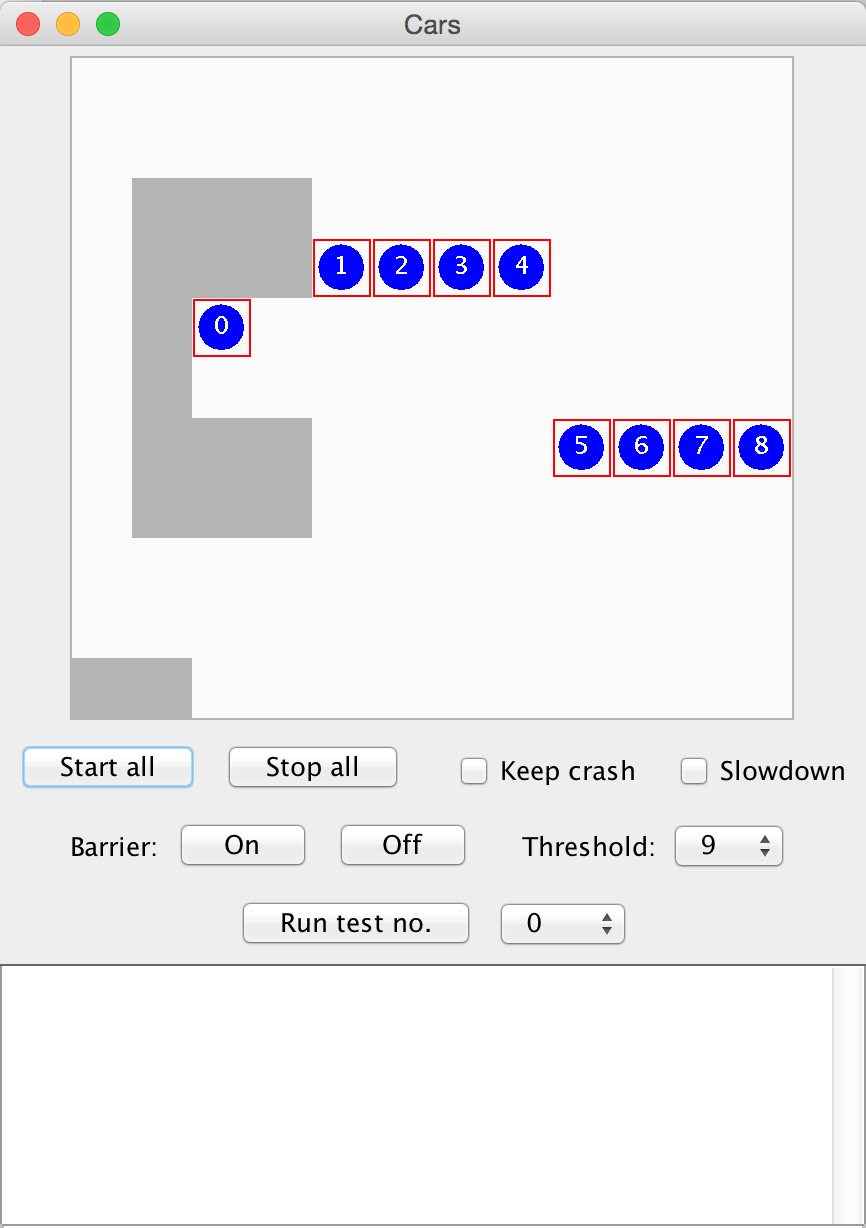
\includegraphics[scale=0.3]{./graphics/Cars1.png}
\end{subfigure}
\begin{subfigure}[b]{0.4\textwidth}
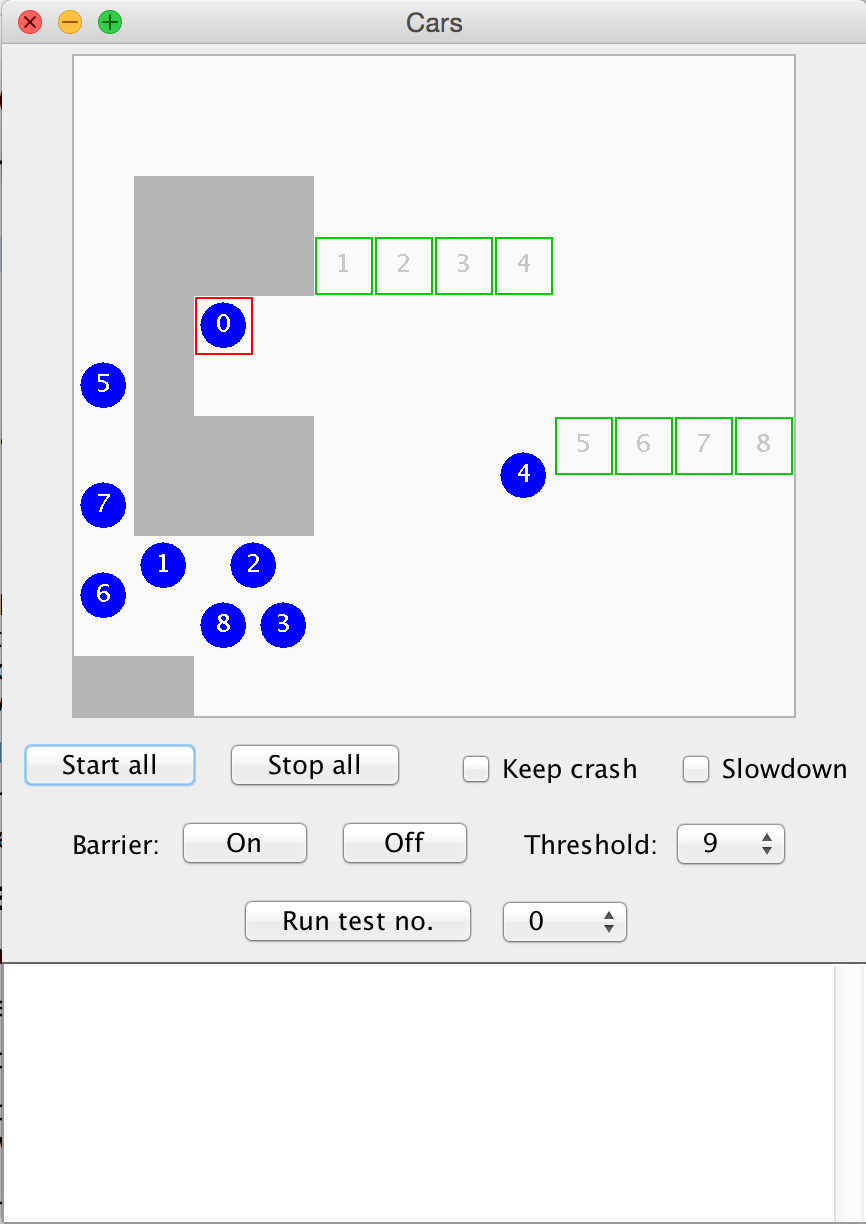
\includegraphics[scale=0.3]{./graphics/Cars2.png}
\end{subfigure}
\end{figure}

The idea behind avoiding collision is that the cars can not move, if another car is either already in the way or both cars are trying to enter same field. The cars will in both cases stop. A car already being an obstacle, the waiting car will have to wait for the other car to move along. This situation will never cause a deadlock, but will have cars waiting for each other in a line.

The other case where two cars want to enter same field, can cause a deadlock with both cars waiting for the other car to move. A solution to the deadlock situation is to have a way to let one of the cars drive on some condition. The condition we have chosen is to let the cars with the highest number advance. The condition will have to be unique, because otherwise the cars will collide. The condition is unique, since no cars have the same number.
\\

One problem with the solution is, when the cars are driving through the alley a direction will stop. The cars driving up the alley will stop for the cars with a higher number. The solution is to let the cars in the alley being prioritized higher, than the cars waiting at the alley.
\\

Unfortunately the collision detection does rarely have a collision on a tile. The collisions happen right, when a faster car want to enter a field, where another car is entering. The faster car will have to ask at the right moment for the collision to happen. The collisions does unfortunately happen. 

A solution would be to use semaphores for every tile in the map to make sure no car would be at the tile at the same time. The cars would then be waiting correctly for the tile to be free. We unfortunately did not notice the issue until late in the project, while we tested other issues. The implementation seemed to work fine while working on step 1, but found out the accidents does happen very rare.

\subsection{Alley}
\subsubsection{Ideas and design}
The idea for the traffic through the alley is to have the cars drive in one direction. If the cars would be driving from both directions, the result would be a deadlock in mid alley. The cars will have to wait for the alley being vacant to change direction. The direction is actually taken by whomever is first to arrive to the alley.

The idea for our alley class is to use semaphores to manage the traffic. The idea is to use 4 different semaphores to manage different aspects of the alley traffic. One semaphore is used to make sure the maximum amount of cars in the alley is no more than 4 cars. A semaphore is used to wait for the traffic being in the specific cars direction. A semaphore is used to make the bottom queue wait for the traffic to become the up direction. The last semaphore is used to make the leave action atomic, which we found necessary due to our spin results.

\subsubsection{Implementation}